\documentclass{article}

%%%%%%%%%%%%%%%%%%%%%%%%%%%%%%%%%%%%%%%%%%%%%%%%%%%%%%%%
% Packages
%%%%%%%%%%%%%%%%%%%%%%%%%%%%%%%%%%%%%%%%%%%%%%%%%%%%%%%%

%\usepackage[utf8]{inputenc} % for overleaf/PLM
\usepackage[latin1]{inputenc} % averil local
\usepackage[T1]{fontenc} % hyphenation
\usepackage{fullpage} % DO NOT USE IN BEAMER
\usepackage[british,UKenglish,USenglish,american]{babel}
%\usepackage{appendix}
\usepackage{amssymb,amsmath,amsthm,enumerate}
\usepackage{mathtools} % coloneqq
%\usepackage{easybmat}
\usepackage{enumitem}
%\usepackage{tikz}
%\usepackage{caption}
\usepackage{float} % [H]
%\usepackage{bbold}
\usepackage[dvipsnames]{xcolor}
\usepackage{stmaryrd} % ll/rr brackets
%\usepackage[notcite, notref]{showkeys}
%\usepackage[tworuled,vlined,nofillcomment]{algorithm2e}
\usepackage[ruled,vlined]{algorithm2e}
%\usepackage{cases} % numbered lines in cases (numcases and subnumcases)
\usepackage[overload]{empheq} % source : https://tex.stackexchange.com/questions/31951/separate-labels-in-cases
\usepackage{caption} % to have subfigures
\usepackage{subcaption} % to have subfigures
\usepackage{cleveref} % \cref. 

%%%%%%%%%%%%%%%%%%%%%%%%%%%%%%%%%%%%%%%%%%%%%%%%%%%%%%%%
% Format
%%%%%%%%%%%%%%%%%%%%%%%%%%%%%%%%%%%%%%%%%%%%%%%%%%%%%%%%

\title{Notes on fixed-point procedure}
\author{} 
\date{}

\SetKwRepeat{Do}{do}{while} % for algorithm2e package, add do-while

% set dashes instead of bullets for item lists
\setlist[itemize,1]{label=$-$}
\setlist[itemize,2]{label=$-$}
\setlist[itemize,3]{label=$-$}

% remove unnecessary formatting of clever references
\crefdefaultlabelformat{(#2#1#3)}
\crefname{equation}{}{}
\crefname{figure}{figure}{Figure}

%%%%%%%%%%%%%%%%%%%%%%%%%%%%%%%%%%%%%%%%%%%%%%%%%%%%%%%%
% Theorems
%%%%%%%%%%%%%%%%%%%%%%%%%%%%%%%%%%%%%%%%%%%%%%%%%%%%%%%%

\newtheorem{proposition}{Proposition}[section]
\newtheorem{definition}{Definition}[section]
\newtheorem{theoreme}{Theorem}[section]
\newtheorem{remarque}{Remark}[section]
\newtheorem{lem}{Lemma}[section]
\numberwithin{equation}{section}

%%%%%%%%%%%%%%%%%%%%%%%%%%%%%%%%%%%%%%%%%%%%%%%%%%%%%%%%
% Commands
%%%%%%%%%%%%%%%%%%%%%%%%%%%%%%%%%%%%%%%%%%%%%%%%%%%%%%%%

\newcommand{\todo}[1]{{\color{red}\textbf{#1}}}
\newcommand{\vv}[1]{\begin{pmatrix} #1 \end{pmatrix}} % vector
\newcommand{\imh}{\textwidth} % meant to be redefined locally

\newcommand{\mysubeq}[2]{ % first argument : label, second : align content
	\begin{subequations}\label{#1}
		\begin{align}[left = {\empheqlbrace}]
			#2
		\end{align}
	\end{subequations}	
}
\newcommand{\mysubcaption}[1]{
	\vspace*{5pt}
	\begin{minipage}{0.8\linewidth}
		\begin{center}
			\footnotesize\emph{#1}
		\end{center}
	\end{minipage}
}
\newcommand{\myproof}[1]{
	\noindent \textbf{Demonstration}
	{\small	#1 \hfill \qedsymbol}
}
\newcommand{\intern}[1]{{\color{RoyalBlue} #1}} % will eventually be removed

% local vocabulary
\newcommand{\ve}{{\overline{v}_e}} % bound on the speed in the support of fe
\newcommand{\we}{{\underline{w}_e}} % transformation of \ve
\newcommand{\DomUpL}{{\mathcal{D}_1}} % domain over the critical char, x=0 side
\newcommand{\DomUpR}{{\mathcal{D}_2}} % domain over the critical char, x=1 side
\newcommand{\DomLow}{{\mathcal{D}_3}} % domain under the critical char + over -\ve
\newcommand{\IntUpL}{{\mathcal{I}_1}} % part of n_i on \DomUpL
\newcommand{\IntUpR}{{\mathcal{I}_2}} % part of n_i on \DomUpR
\newcommand{\IntLow}{{\mathcal{I}_3}} % part of n_i on \DomLow
\newcommand{\domfel}{{\underline{v}}} % lower bound on a segment on which fe >=  \minfe
\newcommand{\domfeu}{{\overline{v}}} % upper bound on a segment on which fe >=  \minfe
\newcommand{\minfe}{{\underline{c}}} % lower bound on f_e on a segment [-\domfeu, -\domfel]
\newcommand{\maxfe}{{\overline{c}}} % upper bound on f_e
\newcommand{\lipfe}{{[f_{e,b}]}} % lipschitz constant of f_{e,b}
\newcommand{\lipfesq}{{[f_{e,b}]_{2}}} % lipschitz constant of f_{e,b}(\sqrt{})

%%%%%%%%%%%%%%%%%%%%%%%%%%%%%%%%%%%%%%%%%%%%%%%%%%%%%%%%
%%%%%%%%%%%%%%%%%%%%%%%%%%%%%%%%%%%%%%%%%%%%%%%%%%%%%%%%
%%%%%%%%%%%%%%%%%%%%%%%%%%%%%%%%%%%%%%%%%%%%%%%%%%%%%%%%

\begin{document}

\maketitle

%Let us define for all $0 < \alpha \leqslant \beta$ the set
%\begin{align*}
%	\mathcal{K}^{\alpha,\beta} \coloneqq \left\{\varphi \in \mathcal{C}^2\left([0,1], \mathbb{R}^{-}\right) \ |\ \varphi(0) = \varphi'(0) = 0, \quad - \beta \leqslant \varphi'' \leqslant - \alpha. \right\}
%\end{align*}
%
%\paragraph{Estimates on the set $\mathcal{K}$}
%
%Since $\varphi : [0,1] \mapsto \mathbb{R}^-$ is decreasing, its inverse $\varphi^{-1} : \mathbb{R}^- \mapsto [0,1]$ is well-defined. By integration and using $\left(\varphi^{-1}\right)' = (\varphi'\circ \varphi^{-1})^{-1}$, we have
%\mysubeq{eq:convex_bounds}{
%	- \beta x &\leqslant \varphi'(x) \leqslant - \alpha x \label{eq:convex_bounds_phiprime} \\
%	- \beta \frac{x^2}{2} &\leqslant \varphi(x) \leqslant - \alpha \frac{x^2}{2} \label{eq:convex_bounds_phi} \\
%	\sqrt{-\frac{2y}{\beta}} &\leqslant \varphi^{-1}(y) \leqslant \sqrt{-\frac{2y}{\alpha}} \label{eq:convex_bounds_phiinv} \\
%	\frac{-1}{\alpha\sqrt{-\frac{2y}{\beta}}} &\leqslant (\varphi^{-1})'(y) \leqslant \frac{-1}{\beta\sqrt{-\frac{2y}{\alpha}}} \label{eq:convex_bounds_phiinv} 
%}

\tableofcontents

% TO WRITE
% What are the characteristics equations
% The choice of the domain $v\leqslant0$ and $x\in[0,1]$
% Symmetries

\section{Notations and assumptions}

We suppose that 
\begin{enumerate}
\item $f_{e,b}$ is nonnegative.
\item $f_{e,b}(v) = f_{e,b}(-v)$ for all $v\in\mathbb{R}$.
\item $f_{e,b}$ satisfies the boundary condition, i.e. $f_{e,b}(v) = 0$ as soon as $\mathcal{L}_e(0,v) \leqslant \mathcal{L}_e(1,0)$.
\item There exists $\maxfe \leqslant 0$ such that $f_{e,b}(v) \leqslant \maxfe$ for all $v \in \mathbb{R}$.
\item There exists $\minfe > 0$ and $0 \leqslant \domfel < \domfeu$ such that $f_{e,b}(v) \geqslant \minfe$ for all $v\in[-\domfeu,-\domfel]$.
\item The function $\varphi$ satisfies $\varphi(0)=\varphi'(0)=0$.
\item The function $\varphi$ is strongly concave, i.e. there exists $\alpha>0$ such that $\varphi((1-\tau) x + \tau y) \geqslant (1-\tau) \varphi(x)+\tau \varphi(y) + \frac{\alpha}{2} (1-\tau)\tau \left|x-y\right|^2$.
\item There exists $\beta > \alpha$ such that $\varphi(1) \geqslant - \beta$. \todo{Uniformly over the fixed-point iterations}
\end{enumerate}

We use the following notations: the Liapunov functions of the electrons and the ions are
\begin{align}\label{eq:def_Le}
	\mathcal{L}_e(x,v) \coloneqq \frac{v^2}{2} - \frac{1}{\mu} \varphi(x).
\end{align}
\begin{align}\label{eq:def_Li}
	\mathcal{L}_i(x,v) \coloneqq \frac{v^2}{2} + \varphi(x).
\end{align}

We define an upper bound $\ve$ over the velocities in the support of $f_e$, given as
\begin{align}\label{eq:def_ve}
	\mathcal{L}_e(0,\ve) \coloneqq \frac{1}{\mu} \beta \geqslant -\frac{1}{\mu}\varphi(1) = \mathcal{L}_e(1,0), \quad\text{i.e.}\quad \ve \coloneqq \sqrt{\frac{2}{\mu}\beta}.
\end{align}

For a given point $(x,v) \in [0,1]\times \mathbb{R}^{-}$, we denote by $(x_b, v_b)$ the intersection of the boundary $\{x\geqslant0,v=0\} \cup \{x=0,v\leqslant 0\}$ with the ion characteristic issued from $(x,v)$. The values are given by
\begin{align}\label{eq:def_xb_vb}
	\vv{x_b(x,v) \\ v_b(x,v)} \coloneqq \vv{\varphi^{-1}\left(\min\left(0,\frac{v^2}{2} + \varphi(x)\right)\right) \\ - \sqrt{\max\left(0,v^2 + 2\varphi(x)\right)}}
%	\begin{cases}
%		\vv{\varphi^{-1}\left(\frac{v^2}{2} + \varphi(x)\right) \\ 0} & \text{if } \mathcal{L}_i(x,v) \leqslant 0, \\
%		\vv{0 \\ - \sqrt{v^2 + 2\varphi(x)}} & \text{if } \mathcal{L}_i(x,v) > 0.
%	\end{cases}
\end{align}


\section{Estimates}

\subsection{Useful elementary lemmas}

\begin{lem}\label{lem:int_1surR_rectangle}
	Let $\alpha>0$, $\overline{x}\geqslant0$ and $\overline{y}\geqslant0$. Then
	\begin{align*}
		\mathcal{I} \coloneqq \int_{x=0}^{\overline{x}} \int_{y=0}^{\overline{y}} \frac{1}{\left(x^2+\alpha y^2\right)^{1/2}} dy dx \leqslant 2 \frac{\sqrt{2\overline{x} \overline{y}}}{\alpha^{1/4}}.
	\end{align*}
\end{lem}

\myproof{
	By the change of variable $z=\sqrt{\alpha} y$, with $\overline{z} \coloneqq \sqrt{\alpha} \overline{y}$, we have
	\begin{align*}
		\mathcal{I} = \frac{1}{\sqrt{\alpha}} \int_{x=0}^{\overline{x}} \int_{z=0}^{\overline{z}} \frac{1}{\left(x^2+ z^2\right)^{1/2}} dz dx.
	\end{align*}
	Notice that $x+z \leqslant \sqrt{2} \left(x^2 + y^2\right)^{1/2}$. Then, 
	\begin{align*}
		\mathcal{I} 
		\leqslant \frac{1}{\sqrt{\alpha}} \int_{x=0}^{\overline{x}} \int_{z=0}^{\overline{z}} \frac{\sqrt{2}}{x+z} dz dx 
		= \sqrt{\frac{2}{\alpha}} \int_{x=0}^{\overline{x}} \ln\left(\frac{x+\overline{z}}{x}\right) dx
		= \sqrt{\frac{2}{\alpha}} \int_{x=0}^{\overline{x}} \ln\left(1 + \frac{\overline{z}}{x}\right) dx.
	\end{align*}
	Using $\ln\left(1+a\right) \leqslant \sqrt{a}$, we get
	\begin{align*}
		\mathcal{I} 
		\leqslant \sqrt{\frac{2}{\alpha}} \int_{x=0}^{\overline{x}} \sqrt{\frac{\overline{z}}{x}} dx 
		= \sqrt{\frac{2}{\alpha}} 2 \sqrt{\overline{x} \overline{z}}
		= 2 \frac{\sqrt{2 \overline{x} \overline{y}}}{\alpha^{1/4}}.
	\end{align*}
}

\intern{
\begin{remarque}[Exact value]
	Let $\overline{r} \coloneqq \sqrt{\overline{x}^2 + \overline{z}^2}$. Then 
	\begin{align*}
		\mathcal{I} = \overline{x} \ln\left(\frac{1 + \overline{z}/\overline{r}}{\overline{x}/\overline{r}}\right) + \overline{z} \ln\left(\frac{1 + \overline{x}/\overline{r}}{\overline{z}/\overline{r}}\right).
	\end{align*}
\end{remarque}
}

\begin{lem}\label{lem:maj_dist_square}
	If $a\geqslant0$ and $b\geqslant0$, then $|a - b| \leqslant \sqrt{|a^2 - b^2|}$.
\end{lem}

\myproof{
	If $a \geqslant b$, then $|a - b| = \sqrt{(a-b)(a-b)} \leqslant \sqrt{(a - b)(a+b)} = \sqrt{a^2 - b^2}$, else $|a-b|=|b-a|$. 
}

\begin{lem}\label{lem:maj_fi}
	Let $\alpha>0$, $L \in \mathbb{R}$ and $0 \leqslant a \leqslant 1$. Suppose that $L + \alpha a^2 \geqslant 0$, and $a>0$ if $L=0$. Then
	\begin{align*}
		\mathcal{I} \coloneqq \int_{z=a}^1 \frac{1}{\left(L + \alpha z^2\right)^{1/2}} dz \leqslant 
%		\begin{cases}
%			\min\left(L^{-1/2},\frac{1+\left(\frac{L}{\alpha}\right)^{1/4}}{\sqrt{\alpha a}}\right) & \text{if } L > 0, \\
%			\frac{1}{\sqrt{\alpha a}} & \text{if } L = 0, \\
%			\min\left(|L|^{-1/2}, \sqrt{\frac{2}{\alpha a}}\right) & \text{if } L < 0.
%		\end{cases}
		\min\left(|L|^{-1/2}, \frac{2}{\sqrt{\alpha a}}\right).
	\end{align*}
%	In particular, we have the uniform bound $\mathcal{I} \leqslant \frac{2}{\sqrt{\alpha a}}$.
\end{lem}

\myproof{
	If $L>0$, we have
	\begin{align*}
		\mathcal{I} = \frac{1}{\sqrt{\alpha}} \int_{z=a}^1 \frac{1}{\left(1 + \left(\sqrt{\frac{\alpha}{L}} z\right)^2\right)^{1/2}} \frac{\sqrt{\alpha} dz}{\sqrt{L}}
		= \frac{1}{\alpha} \int_{w=a \sqrt{\frac{\alpha}{L}}}^{\sqrt{\frac{\alpha}{L}}} \frac{1}{\left(1+w^2\right)^{1/2}} dw 
		= \frac{1}{\sqrt{\alpha}} \left(\sinh^{-1}\left(\sqrt{\frac{\alpha}{L}}\right) - \sinh^{-1}\left(a\sqrt{\frac{\alpha}{L}}\right)\right).
	\end{align*}
	Using the positivity of $\sinh^{-1}\left(a\sqrt{\frac{\alpha}{L}}\right)$, and the coarse estimate $\sinh^{-1}(x) \leqslant x$, we get $\mathcal{I} \leqslant L^{-1/2}$. 
	Moreover, using that $\sinh^{-1}(x) = \log(x + \sqrt{x^2 + 1})$, we get
	\begin{align*}
		\mathcal{I} = \frac{1}{\sqrt{\alpha}} \log\left(\frac{\sqrt{\frac{\alpha}{L}} + \sqrt{\frac{\alpha}{L} + 1}}{a\sqrt{\frac{\alpha}{L}} + \sqrt{a^2\frac{\alpha}{L} + 1}}\right)
		= \frac{1}{\sqrt{\alpha}} \log\left(\frac{1 + \sqrt{1 + \frac{L}{\alpha}}}{a + \sqrt{a^2 + \frac{L}{\alpha}}}\right)
		\leqslant \frac{1}{\sqrt{\alpha}} \log\left(\frac{2 + \sqrt{\frac{L}{\alpha}}}{2 a}\right)
		\leqslant \frac{1 + \left(\frac{L}{\alpha}\right)^{1/4}}{\sqrt{\alpha a}}.
	\end{align*}
	\intern{I shamelessly used $\frac{1}{2} \leqslant 1$.} Then $\mathcal{I} \leqslant \min\left(L^{-1/2},\frac{1 + \left(\frac{L}{\alpha}\right)^{1/4}}{\sqrt{\alpha a}}\right)$ on $L>0$. But whenever $L \geqslant \alpha$, the min is attained in its first argument: indeed, $L^{-1/2} \leqslant \frac{1}{\sqrt{\alpha a}} \leqslant \frac{1+\left(\frac{L}{\alpha}\right)^{1/4}}{\sqrt{\alpha a}}$. Then we obtained $\mathcal{I} \leqslant \min(L^{-1/2},\frac{2}{\sqrt{\alpha a}})$ on $L>0$.
	If $L=0$, we have
	\begin{align*}
		\int_{z=a}^1 \frac{1}{\sqrt{\alpha} z} dz = \frac{\log(1/a)}{\sqrt{\alpha}} \frac{2}{\sqrt{\alpha a}}.
	\end{align*}
	Finally, if $L<0$, the integral becomes
	\begin{align*}
		\mathcal{I} = \frac{1}{\sqrt{\alpha}} \int_{a}^1 \frac{1}{\left(\left(\sqrt{\frac{\alpha}{|L|}} z\right)^2-1\right)^{1/2}} \frac{\sqrt{\alpha} dz}{\sqrt{|L|}}
		= \frac{1}{\alpha} \int_{a \sqrt{\frac{\alpha}{|L|}}}^{\sqrt{\frac{\alpha}{|L|}}} \frac{1}{\left(w^2-1\right)^{1/2}} dw 
		= \frac{\cosh^{-1}\left(\sqrt{\frac{\alpha}{|L|}}\right) - \cosh^{-1}\left(a\sqrt{\frac{\alpha}{|L|}}\right)}{\sqrt{\alpha}}.
	\end{align*}
	The expression is well-defined, since $L + \alpha a^2 \geqslant 0$ implies $a \sqrt{\frac{\alpha}{-L}} \geqslant 1$ when $-L>0$.
	Since $\cosh^{-1}(x) \leqslant x$, we obtain the coarse estimate $\mathcal{I} \leqslant |L|^{-1/2}$.
	Using that $\cosh^{-1}(x)=\log\left(x+\sqrt{x^2-1}\right)$, we get
	\begin{align*}
		\mathcal{I} 
		= \frac{1}{\sqrt{\alpha}} \log\left(\frac{1 + \sqrt{1 - \frac{|L|}{\alpha}}}{a + \sqrt{a^2 - \frac{|L|}{\alpha}}}\right) 
		\leqslant \frac{1}{\sqrt{\alpha}} \log\left(\frac{2}{a}\right) 
		\leqslant \sqrt{\frac{2}{\alpha a}}
		\leqslant \frac{2}{\sqrt{\alpha a}}.
	\end{align*}
	
%	To obtain the uniform bound, we just have to show that for all $L > 0$,
%	\begin{align*}
%		L^{-1/2} \textbf{1}_{\{L > c\}} + \frac{1+\left(\frac{L}{\alpha}\right)^{1/4}}{\sqrt{\alpha a}} \textbf{1}_{\{L \leqslant c\}}
%		\coloneqq \min\left(L^{-1/2},\frac{1+\left(\frac{L}{\alpha}\right)^{1/4}}{\sqrt{\alpha a}}\right) 
%		\leqslant \frac{2}{\sqrt{\alpha a}}.
%	\end{align*}
%	Notice that $L \geqslant \alpha$ implies $L^{-1/2} \leqslant \frac{1}{\sqrt{\alpha a}} \leqslant \frac{1+\left(\frac{L}{\alpha}\right)^{1/4}}{\sqrt{\alpha a}}$, so that $c \leqslant \alpha$, and the restriction $\frac{1+\left(\frac{L}{\alpha}\right)^{1/4}}{\sqrt{\alpha a}} \textbf{1}_{\{L \leqslant c\}}$ is bounded by $\frac{2}{\sqrt{\alpha a}}$. On the other hand, the inequality $L^{-1/2} \leqslant \frac{2}{\sqrt{\alpha a}}$ is satisfied as soon as $\frac{\alpha a}{4} \leqslant L$, and the critical case $L=\frac{\alpha a}{4}$ yields
%	\begin{align*}
%		\frac{1+\left(\frac{\alpha a}{4 \alpha}\right)^{1/4}}{\sqrt{\alpha a}} < \frac{2}{\sqrt{\alpha a}} = L^{-1/2}.
%	\end{align*}
%	Then $c \geqslant \frac{\alpha a}{4}$, and the bound is uniform in $L$.
}

\subsection{Properties of the electron density $n_e$}

\begin{lem}\label{lem:ne_continuous_space}
	The electron density $n_e$ is bounded and continuous.
\end{lem}

\myproof{
	For each $0\leqslant x \leqslant y \leqslant 1$, we define the velocity $v_x(y) \geqslant 0$ such that 
	\begin{align*}
		\mathcal{L}_e(x,v_x(y)) = \mathcal{L}_e(y,0) \quad \iff \quad v_x(y) = \left(\frac{2}{\mu}\left(\varphi(x) - \varphi(y)\right)\right)^{1/2}.
	\end{align*} 
	In particular, owing to the boundary conditions, the function $v \to f_e(x,v)$ vanishes for $|v| \geqslant v_x(1)$. Then
	\begin{align*}
		n_e(x) = \int_{v=-v_x(1)}^{v_x(1)} f_e(x,v) dv \leqslant 2 \maxfe v_x(1) = 2 \maxfe \left(\frac{2}{\mu} (\varphi(x) - \varphi(1))\right)^{1/2} \leqslant 2 \maxfe \sqrt{\frac{2\beta}{\mu}}.
	\end{align*}
	
	Moreover, using the symmetry $f_e(x,v) = f_e(x,-v)$, we may write
	\begin{align*}
		n_e(x) - n_e(y) = 2 \underbrace{\int_{v=0}^{v_x(y)} f_e(x,v) dv}_{\eqqcolon\,\mathcal{I}^+} + 2 \left(\underbrace{\int_{v=v_x(y)}^{v_x(1)}  f_e(x,v) dv - \int_{v=0}^{v_y(1)} f_e(y,v) dv}_{\eqqcolon\,\mathcal{I}^-}\right).
	\end{align*}
	The term $\mathcal{I}^+$ is bounded by $\maxfe v_x(y) = \maxfe \left(\frac{2}{\mu}\left(\varphi(x) - \varphi(y)\right)\right)^{1/2}$, and by continuity of $\varphi$, we have $\mathcal{I}^{+} \underset{y\to x}{\longrightarrow} 0$. On the first integral of $\mathcal{I}^{-}$, we apply the change of variable
	\begin{align*}
		w = \left(v^2 - \frac{2}{\mu} \left(\varphi(x) - \varphi(y)\right)\right)^{1/2} \quad \iff \quad dv = \frac{w}{\left(w^2 + \frac{2}{\mu}\left(\varphi(x) - \varphi(y)\right)\right)^{1/2}} \,dw, \quad w \in [0,v_y(1)]
	\end{align*}
	to get
	\begin{align*}
		\mathcal{I}^- = \int_{w=0}^{v_y(1)} f_e\left(x,\left(w^2 + \frac{2}{\mu}\left(\varphi(x) - \varphi(y)\right)\right)^{1/2}\right) \frac{w}{\left(w^2 + \frac{2}{\mu}\left(\varphi(x) - \varphi(y)\right)\right)^{1/2}} dw - \int_{v=0}^{v_y(1)} f_e(y,v) dv.
	\end{align*}
	Notice that
	\begin{align*}
		f_e\left(x,\left(w^2 + \frac{2}{\mu}\left(\varphi(x) - \varphi(y)\right)\right)^{1/2}\right)
		= f_{e,b} \left(\frac{w^2}{2} + \frac{1}{\mu}\left(\varphi(x) - \varphi(y)\right) - \frac{1}{\mu} \varphi(x)\right)
		= f_e(y,w).
	\end{align*}
	Renaming $w$ in $v$, we obtain the (clearly nonpositive) expression
	\begin{align*}
		\mathcal{I}^- 
		&= \int_{v=0}^{v_y(1)} f_e(y,v) \left(\frac{v}{\left(v^2 + \frac{2}{\mu}\left(\varphi(x) - \varphi(y)\right)\right)^{1/2}} - 1\right) dv 
		\geqslant \maxfe \int_{v=0}^{v_y(1)}\left(\frac{v}{\left(v^2 + \frac{2}{\mu}\left(\varphi(x) - \varphi(y)\right)\right)^{1/2}} - 1\right) dv \\
		&= \maxfe \left(\left(v_y(1)^2 + \frac{2}{\mu}\left(\underbrace{\varphi(x) - \varphi(y)}_{\geqslant 0}\right)\right)^{1/2} - \left(\frac{2}{\mu}\left(\varphi(x) - \varphi(y)\right)\right)^{1/2} - v_y(1)\right) 
		\geqslant - \maxfe \left(\frac{2}{\mu}\left(\varphi(x) - \varphi(y)\right)\right)^{1/2}
	\end{align*}
	and this shows that $\mathcal{I}^{-} \underset{y\to x}{\longrightarrow} 0$.
}

\begin{lem}\label{lem:ne_continuous_phi}
	Let $n_e^{\varphi}$ and $n_e^{\psi}$ be the electron densities generated by potentials $\varphi$ and $\psi$ satisfying the assumptions. Then
	\begin{enumerate}
	\item If $f_{e,b}$ is Lipschitz-continuous with constant $\lipfe$, then 
	\begin{align*}
		|n_e^{\varphi}(x) - n_e^{\psi}(x)| \leqslant 2 \lipfe \ve \sqrt{\frac{2}{\mu}}\left|\varphi(x) -\psi(x)\right|^{1/2} \quad \forall (x,y) \in [0,1]^2.
	\end{align*}
	\item If there exists a constant $[f_{e,b}]$ such that $|f_{e,b}(x) - f_{e,b}(y)| \leqslant [f_{e,b}] |x^2 - y^2|$ \intern{(or equivalently, $x \to f_{e,b}(\sqrt{x})$ is a lipschitz function, as for instance $e^{-x^2}$)}, then 
	\begin{align*}
		|n_e^{\varphi}(x) - n_e^{\psi}(x)| \leqslant \frac{4\ve \lipfesq}{\mu} \left|\varphi(x) - \psi(x)\right| \quad \forall (x,y) \in [0,1]^2.
	\end{align*}
	\end{enumerate}
\end{lem}

\myproof{
	We have
	\begin{align*}
		\left|n_e^{\varphi}(x) - n_e^{\psi}(x)\right| 
		\leqslant 2 \int_{v=0}^{\ve} \left|f_e^{\varphi}(x,v) - f_e^{\psi}(x,v)\right| dv
		= 2 \int_{v=0}^{\ve} \left|f_{e,b}\left(\left(v^2 - \frac{2}{\mu}\varphi(x)\right)^{1/2}\right) - f_{e,b}\left(\left(v^2 - \frac{2}{\mu}\psi(x)\right)^{1/2}\right)\right| dv.
	\end{align*}
	Then, if $f_{e,b}$ is Lipschitz with constant $\lipfe$, we obtain
	\begin{align*}
		\left|n_e^{\varphi}(x) - n_e^{\psi}(x)\right| \leqslant 2 \lipfe \int_{v=0}^{\ve} \left|\left(v^2 - \frac{2}{\mu}\varphi(x)\right)^{1/2} - \left(v^2 - \frac{2}{\mu}\psi(x)\right)^{1/2}\right| dv.
	\end{align*} 
	Using \cref{lem:maj_dist_square} yields
	\begin{align*}
		\left|n_e^{\varphi}(x) - n_e^{\psi}(x)\right| 
		\leqslant 2 \lipfe \int_{v=0}^{\ve} \left|- \frac{2}{\mu}\varphi(x) + \frac{2}{\mu}\psi(x)\right|^{1/2} dv
		= 2 \lipfe \ve \sqrt{\frac{2}{\mu}}\left|\varphi(x) -\psi(x)\right|^{1/2}.
	\end{align*}
	If $f_{e,b}(\sqrt{\cdot})$ is Lipschitz with constant $\lipfesq$, we may directly write
	\begin{align*}
		\left|n_e^{\varphi}(x) - n_e^{\psi}(x)\right| \leqslant 2 \ve \lipfesq \frac{2}{\mu} \left|\varphi(x) - \psi(x)\right|.
	\end{align*} 
}

\subsection{Properties of the ion density $n_i$}

The estimates will rely on two particular cases, the we treat independently as lemmas. For a given $x$, we define $g_x : [0,x] \mapsto \mathbb{R}^{+}$ by
\begin{align*}
	\mathcal{L}_i(x,-g_x(y)) = \mathcal{L}_i(y,0), \quad \text{i.e.} \quad g_x(y) = \left(2\left(\varphi(y) - \varphi(x)\right)\right)^{1/2}.
\end{align*}

\begin{lem}\label{lem:upperbound_ni_endchar}
	Let $0\leqslant y < x \leqslant 1$. We have
	\begin{align*}
		\mathcal{I} \coloneqq \int_{v=-g_x(y)}^{0} \int_{z = x_b(x,v)}^{x} \frac{1}{\left(v^2-g_x^2(z)\right)^{1/2}} dz\,dv \leqslant 2 \sqrt{\frac{2}{\alpha}}\left(\varphi(y) - \varphi(x)\right)^{1/4} \sqrt{x-y}. 
	\end{align*}
\end{lem}

\myproof{
	Let us first use Fubini's theorem to switch the order of integration. The lower bound $x_b(x,v) \geqslant z$ becomes an upper bound $v \leqslant -g_x(z)$, and we have
	\begin{align*}
		\mathcal{I} 
		= \int_{z=y}^{x} \int_{v = -g_x(y)}^{-g_x(z)} \frac{1}{\left(v^2-g_x^2(z)\right)^{1/2}} dv\,dz 
		= \int_{z=y}^{x} \int_{v = g_x(z)}^{g_x(y)} \frac{1}{\left(v^2-g_x^2(z)\right)^{1/2}} dv\,dz.
	\end{align*} 
	With the change of variable $w = v - g_x(z)$, and using $\frac{d}{dw} \left[\sinh^{-1}\left(\sqrt{\frac{w}{a}}\right)\right] = \left(w^2 + 2aw\right)^{-1/2}$, we get
	\begin{align*}
		\mathcal{I} 
		= \int_{z=y}^{x} \int_{w = 0}^{g_x(y)-g_x(z)} \frac{1}{\left(w^2 + 2 w g_x(z)\right)^{1/2}} dw\,dz
		= \int_{z=y}^{x} \sinh^{-1}\left(\sqrt{\frac{g_x(y) -g_x(z)}{g_x(z)}}\right) dz.
	\end{align*}
	Using the coarse estimates $\sinh^{-1}(a) \leqslant a$ and $\sqrt{\frac{a-b}{b}} \leqslant \sqrt{\frac{a}{b}}$, we get
	\begin{align*}
		\mathcal{I} \leqslant \int_{z=y}^{x} \sqrt{\frac{g_x(y)}{g_x(z)}} dz = \int_{z=y}^{x} \left(\frac{\varphi(y) - \varphi(x)}{\varphi(z) - \varphi(x)}\right)^{1/4} dz.
	\end{align*}
	The assumption of strong concavity yields $\varphi(z) - \varphi(x) \geqslant - \varphi'(z) (x - z) + \frac{\alpha}{2} |x - z|^2 \geqslant \frac{\alpha}{2} (x - z)^2$, so that 
	\begin{align*}
		\mathcal{I} 
		\leqslant \sqrt{\frac{2}{\alpha}}\left(\varphi(y) - \varphi(x)\right)^{1/4} \int_{z=y}^{x} \frac{1}{\left(x - z\right)^{1/2}} dz 
		= 2 \sqrt{\frac{2}{\alpha}}\left(\varphi(y) - \varphi(x)\right)^{1/4} \sqrt{x-y}.
	\end{align*}
}

\begin{lem}\label{lem:upperbound_ni_beginchar}
	Let $0 \leqslant y \leqslant x \leqslant 1$, and $-v_0 < -g_x(y)$. We have
	\begin{align*}
		\mathcal{I} \coloneqq \int_{v=-v_0}^{-g_x(y)} \int_{z=y}^{1} \frac{1}{\left(v^2 + 2 \left(\varphi(x) - \varphi(z)\right)\right)^{1/2}} dz \, dv \leqslant \frac{2\sqrt{2(1-y)}}{\alpha^{1/4}} \left(v_0^2 + 2 \left(\varphi(x) - \varphi(y)\right)\right)^{1/4}.
	\end{align*}
\end{lem}

\myproof{
	We first shift the $v-$integration from the vertical line $z=x$ to $z=y$. Let $w = w(v)$ be such that
	\begin{align*}
		\mathcal{L}_i(y,w(v)) = \mathcal{L}_i(x,v), \quad \text{i.e.} \quad w(v) = -\left(v^2 + 2 \left(\varphi(x) - \varphi(y)\right)\right), \text{ and } dv = \frac{-w}{\left(w^2 + 2 \left(\varphi(y) - \varphi(x)\right)\right)^{1/2}}  dw.
	\end{align*}
	Then, defining $w_0 \coloneqq \left(v_0^2 + 2 \left(\varphi(x) - \varphi(y)\right)\right)^{1/2}$, and noticing that $w(-g_x(y)) = 0$, we get
	\begin{align*}
		\mathcal{I} = \int_{w=-w_0}^{0} \int_{z=y}^{1} \frac{1}{\left(w^2 + 2 \left(\varphi(y) - \varphi(z)\right)\right)^{1/2}} dz \frac{-w}{\left(w^2 + 2 \left(\varphi(y) - \varphi(x)\right)\right)^{1/2}} dw.
	\end{align*}
	Since $y \leqslant x$, we have $\varphi(y) \geqslant \varphi(x)$, and $\frac{-w}{\left(w^2 + 2 \left(\varphi(y) - \varphi(x)\right)\right)^{1/2}} \leqslant \frac{-w}{|w|} = 1$. By the strong concavity assumption, we have $\varphi(y) - \varphi(z) \geqslant - \varphi'(y) (z - y) + \frac{\alpha}{2} |z - y|^2 \geqslant \frac{\alpha}{2} (z - y)^2$, so that
	\begin{align*}
		\mathcal{I} \leqslant \int_{w=-w_0}^{0} \int_{z=y}^{1} \frac{1}{\left(w^2 + \alpha (z- y)^2\right)^{1/2}} dz dw = \int_{w=0}^{w_0} \int_{z=0}^{1-y} \frac{1}{\left(w^2 + \alpha z^2\right)^{1/2}} dz dw.
	\end{align*}
	Using \cref{lem:int_1surR_rectangle}, we conclude that 
	\begin{align*}
		\mathcal{I} \leqslant 2 \frac{\sqrt{2 w_0 (1-y)}}{\alpha^{1/4}} = \frac{2\sqrt{2(1-y)}}{\alpha^{1/4}} \left(v_0^2 + 2 \left(\varphi(x) - \varphi(y)\right)\right)^{1/4}.
	\end{align*}
}

\begin{proposition}
	The density $n_i$ is bounded by a constant depending on $\varphi$ only through $\varphi(1)$.
\end{proposition}

\myproof{
	We use the symmetry of $f_i$ to write
	\begin{align*}
		n_i(x) = \int_{v=-\infty}^{\infty} f_i(x,v) dv = 2 \int_{v=-\infty}^{0} f_i(x_b(x,v), v_b(x,v)) dv = 2 \int_{v=-\infty}^{0} \int_{t=-\infty}^{0} f_e(x(t),v(t)) dt dv,
	\end{align*}
	where $(x(t),v(t))_{t\leqslant0}$ is the ion characteristic reaching $(x_b(x,v),v_b(x,v))$ at $t=0$. Notice that the lower bounds are artificial, since the characteristic enters the support of $f_e$ in finite time: we may use $v \geqslant -\ve$, and consider only times $t$ for which $x(t) \in [0,1]$. 
	
	We first reparametrize $(x(t),v(t))$ using the space variable. Define $z = x(t) \in[x_b,1]$, and observe that
	\begin{align*}
		dz = \dot{x}(t) dt = v(t) dt, \quad \text{with}\quad \mathcal{L}_i(z,v(t)) = \mathcal{L}_i(x,v) \quad\iff\quad v(t) = -\left(v^2 + 2\left(\varphi(x) - \varphi(z)\right)\right)^{1/2}.
	\end{align*}
	Then, the density rewrites
	\begin{align*}
		n_i(x) = 2 \int_{v=-\ve}^{0} \int_{z=x_b(x,v)}^{1} \frac{f_e\left(z, -\left(v^2 + 2\left(\varphi(x) - \varphi(z)\right)\right)^{1/2}\right)}{\left(v^2 + 2\left(\varphi(x) - \varphi(z)\right)\right)^{1/2}} \, dz dv.
	\end{align*}
	Let us show that $n_i$ is bounded. We use the coarse estimate $f_e \leqslant \maxfe$, and decompose the integral in three:
	\begin{align*}
		n_i(x) \leqslant 2 \maxfe \left[
		\underbrace{\int_{v=-g_x(0)}^{0} \int_{z=x_b(x,v)}^{x}}_{\IntUpL} + 
		\underbrace{\int_{v=-g_x(0)}^{0} \int_{z=x}^{1}}_{\IntUpR} + 
		\underbrace{\int_{v=-\ve}^{-g_x(0)} \int_{z=x_b(x,v)}^{1}}_{\IntLow} \right] 
		\frac{1}{\left(v^2 + 2\left(\varphi(x) - \varphi(z)\right)\right)^{1/2}} \, dz dv.
	\end{align*}
	The corresponding domains are represented \cref{fig:charmaps_domainmap}. 
	\begin{figure}
		\centering
		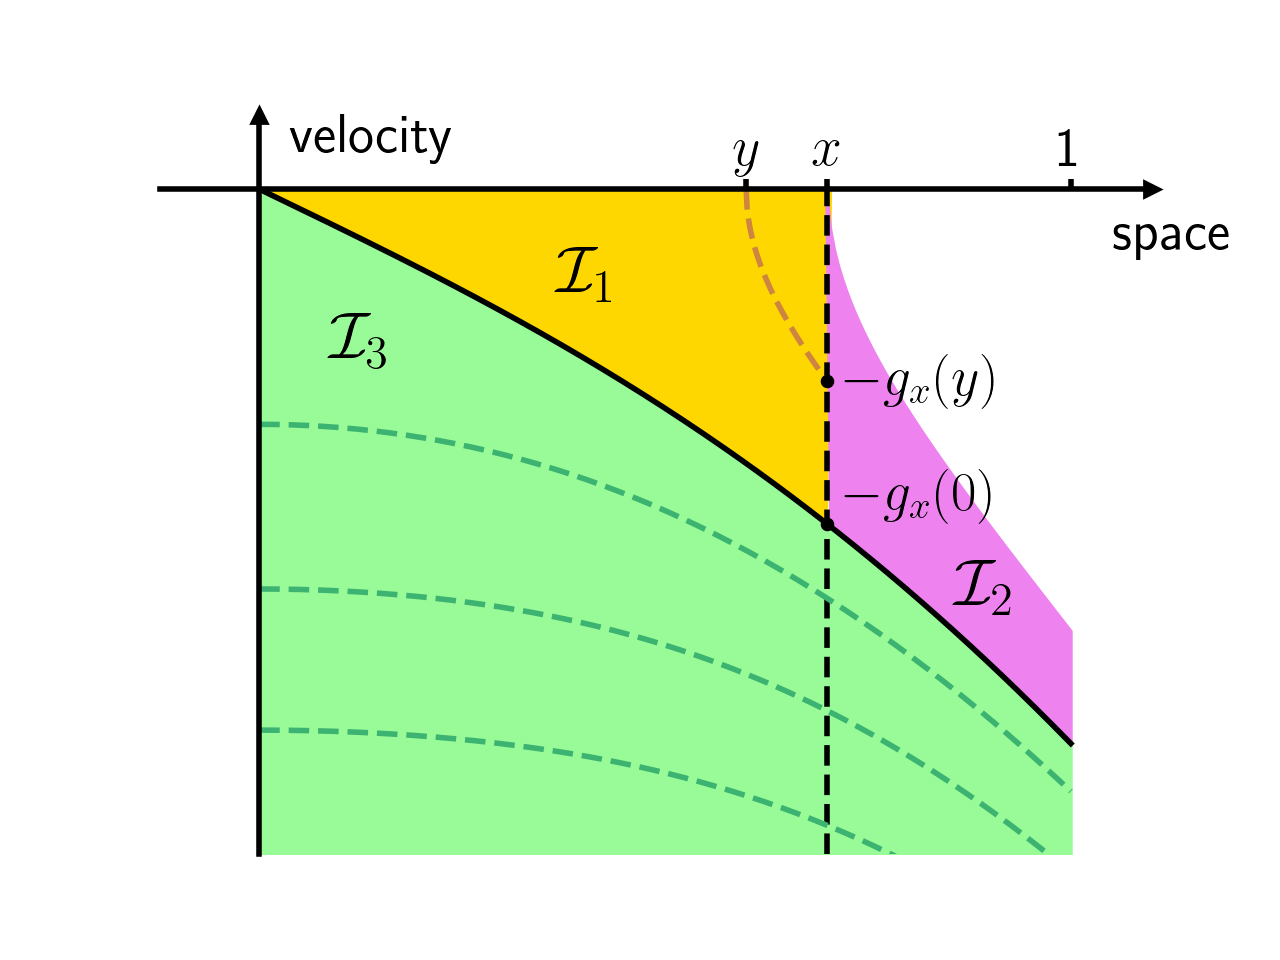
\includegraphics[width=0.5\linewidth]{images/fpcharmaps_domainmap}
		\caption{Decomposition of the integral defining $n_i$.}
		\mysubcaption{The phase space is divided by the critical characteristic (in solid black). Whenever $v\leqslant -g_x(0)$, the characteristics (dotted green lines) are reaching the boundary with $x_b(x,v)=0$. }
		\label{fig:charmaps_domainmap}
	\end{figure}
	
	
	Notice that whenever $z \leqslant x$, we have $0 \geqslant 2\left(\varphi(x) - \varphi(z)\right) = - \left(2\left(\varphi(z) - \varphi(x)\right)\right)^{2/2} = - g_x^2(z)$. Then, the integral $\IntUpL$ may be bounded using \cref{lem:upperbound_ni_endchar} with $y=0$:
	\begin{align*}
		\IntUpL = \int_{v=-g_x(0)}^{0} \int_{z=x_b(x,v)}^{x} \frac{1}{\left(v^2 - g_x^2(z)\right)^{1/2}} \, dz dv 
		\leqslant 2 \sqrt{\frac{2}{\alpha}} \left(-\varphi(x)\right)^{1/4} \sqrt{x}
		\leqslant 2 \sqrt{\frac{2}{\alpha}} \left(-\varphi(1)\right)^{1/4}.
	\end{align*}
	
	We use \cref{lem:upperbound_ni_beginchar} to bound $\IntUpR$ and $\IntLow$. In the first case, we take $y=x$ and $v_0 = g_x(0)$, and notice that $-g_x(x)=0$. In the second case, we take $v_0 = \ve$ and $y=0$, and notice that on $v \leqslant -g_x(0)$, we have $x_b(x,v) = 0$ (the velocity is low enough so that the characteristic ends on $x_b=0$). This yields
	\begin{align*}
		\IntUpR \leqslant \frac{2\sqrt{2(1-x)}}{\alpha^{1/4}} \left(g_x^2(0)\right)^{1/4} \leqslant \frac{4}{\alpha^{1/4}} \left(-\varphi(1)\right)^{1/2} , \quad\text{and}\quad
		\IntLow \leqslant \frac{2\sqrt{2}}{\alpha^{1/4}} \left(\ve^2 + 2 \varphi(x)\right)^{1/4} \leqslant \frac{4}{\alpha^{1/4}} \left(\frac{\beta}{\mu}\right)^{1/4}.
	\end{align*}
}

\begin{proposition}
	The density $n_i$ is continuous. 
\end{proposition}

\myproof{
	Let $0 \leqslant y < x \leqslant 1$. For convenience, we represent $n_i(x)$ (resp. $n_i(y)$) as an integral with the artificial lower bound $-g_x(-\ve) \leqslant -\ve$ (resp. $-g_y(-\ve)$). Then
	\begin{align}\label{eq:def_ni_sym}
		n_i(x) - n_i(y) 
		&= 2 \int_{v=-g_x(-\ve)}^0 f_i(x_b(x,v),v_b(x,v)) dv - 2 \int_{v=-g_y(-\ve)}^0 f_i(x_b(y,v),v_b(y,v)) dv \\
		&= 2 \underbrace{\left[\int_{v=-g_x(-\ve)}^{-g_x(y)} f_i(x_b(x,v),v_b(x,v)) dv - \int_{v=-g_y(-\ve)}^{0} f_i(x_b(y,v),v_b(y,v)) dv\right]}_{\eqqcolon\,\mathcal{I}^-}
		+ 2 \underbrace{\int_{v=-g_x(y)}^{0} f_i(x_b(x,v),v_b(x,v)) dv}_{\eqqcolon\,\mathcal{I}^+}.
	\end{align}

	The term $\mathcal{I}^+$ is clearly nonnegative, and may be adressed using our lemmas. Indeed, using the integral representation of $f_i(x_b,v_b)$ and the reparametrization by a space variable $z$, we have
	\begin{align*}
		\mathcal{I}^+ 
		&= \int_{v=-g_x(y)}^{0} \left[\int_{z=x_b(x,v)}^{x} + \int_{z=x}^{1}\right] \frac{f_e(z,-\left(v^2+2\left(\varphi(x)-\varphi(z)\right)\right)^{1/2}))}{\left(v^2+2\left(\varphi(x)-\varphi(z)\right)\right)^{1/2}} \,dz dv \\
		&\leqslant \maxfe \int_{v=-g_x(y)}^{0} \int_{z=x_b(x,v)}^{x} \frac{1}{\left(v^2-g_x^2(z)\right)^{1/2}} \, dz dv + \maxfe \int_{v=-g_x(y)}^{0} \int_{z=x}^{1} \frac{1}{\left(v^2+2\left(\varphi(x)-\varphi(z)\right)\right)^{1/2}} \,dz dv \\
		&\leqslant \maxfe \left(2\sqrt{\frac{2}{\alpha}} \left(\varphi(y)-\varphi(x)\right)^{1/4} \sqrt{x-y} + \frac{2\sqrt{2}}{\alpha^{1/4}} \left(2(\varphi(y)-\varphi(x))\right)^{1/2}\right),
	\end{align*}
	where we used \cref{lem:upperbound_ni_endchar} for the first term, and \cref{lem:upperbound_ni_beginchar} for the second term (with $y=x$ and $v_0 = -g_x(y)$ under the notations of the lemma). Since $\varphi$ is continuous, we deduce that $\mathcal{I}^{+} \underset{y\to x}{\longrightarrow} 0$. Taking the extreme case $y=0$ and $x=1$, we obtain that 
	\begin{align*}
		\mathcal{I}^+ \leqslant \maxfe \left(2\sqrt{\frac{2}{\alpha}} \left(-\varphi(1)\right)^{1/4} + \frac{2\sqrt{2}}{\alpha^{1/4}} \left(-2\varphi(1)\right)^{1/2}\right) \eqqcolon K.
	\end{align*}

	Let us now focus on $\mathcal{I}^-$. On the first integral, we make the change of variable
	\begin{align*}
		w = -\left(v^2 + 2 \left(\varphi(x) - \varphi(y)\right)\right)^{1/2} \quad v = -\left(w^2 + 2 \left(\varphi(y) - \varphi(x)\right)\right)^{1/2}.
	\end{align*}
	Since $\mathcal{L}_i(x,v) = \mathcal{L}_i(y,w)$, this yields $x_b(x,v) = x_b(y,w)$ and $v_b(x,v) = v_b(y,w)$. The bounds $v\in[-g_x(-\ve),-g_x(y)]$ are exactly transported to $w\in[-g_y(-\ve),0]$. Renaming $w$ in $v$, we get
	\begin{align*}
		\mathcal{I}^- = \int_{v=-g_y(-\ve)}^{0} f_i(x_b(y,v),v_b(y,v)) \left(\frac{-v}{\left(v^2 + 2 \left(\varphi(y) - \varphi(x)\right)\right)^{1/2}} - 1\right) dv.
	\end{align*}
	Since $\varphi(y) \geqslant \varphi(x)$, the factor of $f_i$ is nonpositive, and so is $\mathcal{I}^-$. Moreover, 
	\begin{align*}
		n_i(x) - n_i(y) = 2 \mathcal{I}^- + 2\mathcal{I}^+ \leqslant 2 \mathcal{I}^{-} + 2 K \quad\iff\quad \mathcal{I}^- = - K + n_i(x) - n_i(y) \geqslant - K - |n_i|_{\infty}
	\end{align*}
	and $\mathcal{I}^-$ is bounded. The function $\frac{-v}{\left(v^2 + 2 \left(\varphi(y) - \varphi(x)\right)\right)^{1/2}} - 1$ converges pointwise to 0 when $x\to y$ \todo{and $f_i$ is almost everywhere finite}, and by Lebesgue's dominated convergence, $\mathcal{I}^- \underset{x\to y}{\longrightarrow} 0$. Then $n_i$ is continuous.
}

\todo{
In the future:
\begin{itemize}
\item Now that we have estimates, write it in function of $\alpha$ and $\beta$, and see how to get stability of the set of strongly concave functions satisfying all the hypotheses by the Poisson problem (essentially, find tweaks of $\lambda$, $\mu$, $\nu$, $\alpha$ and/or $\beta$ such that the estimates are propagated).
\item If $f_{e,b}$ vanishes in a neighbourhood of $(0,0)$ (or decreases fast enough, see how fast), show that $f_i$ is bounded.
\item Under that same assumption, we should obtain stronger continuity over $n_i$, and $n_i$ may be continuous with respect to $\varphi$ (in the same sense as $n_e$ in \cref{lem:ne_continuous_phi}).
\item If the estimates with respect to $|\varphi - \psi|_{\infty}$ succeed, define numerical scheme and see what we cas say about it.
\end{itemize}
}

\begin{lem}
	The density $n_i$ is bounded away from 0 uniformly over $x\in[0,1]$.
\end{lem}

\myproof{
	By assumption, there exists a constant $\minfe>0$ such that $f_{e,b} (v) \geqslant \minfe \textbf{1}_{\left\{\domfel \leqslant |v| \leqslant \domfeu\right\}}$, which implies
	\begin{align*}
		f_e(x,v) \geqslant \minfe \textbf{1}_{\left\{\mathcal{L}_e(0,\domfel) \leqslant \mathcal{L}_e(x,v) \leqslant \mathcal{L}_e(0,\domfeu)\right\}}.
	\end{align*}
	Let $g_x : \mathbb{R}^{-} \mapsto \mathbb{R}^+$ be such that $\mathcal{L}_i(0,v) = \mathcal{L}_i(x,-g_x(v))$. As in \cref{eq:def_ni_sym}, we define $n_i(x)$ by an integral over $v\in\mathbb{R}^{-} = ]-\infty,-g_x(0)] \cup ]-g_x(0),0]$. Since we want an uniform lower bound, we will sacrify the (nonnegative) integral on $]-g_x(0),0]$. Moreover, 
	\begin{align*}
		w \leqslant -g_x(-\domfeu) \quad\implies\quad \mathcal{L}_i(0,v_b(x,w)) = \mathcal{L}_i(x,w) \geqslant \mathcal{L}_i(x,-g_x(-\domfeu)) = \mathcal{L}_i(0,-\domfeu) = \mathcal{L}_e(0,\domfeu),
	\end{align*}
	and $f_e$ vanishes identically along the ion characteristic crossing $(x,w)$. Then, we may restrict the $w-$integral over the domain $[-g_x(-\domfeu),-g_x(0)]$ for all $x$, and write
	\begin{align*}
		n_i(x) \geqslant \int_{w=-g_x(-\domfeu)}^{-g_x(0)} f_i(0,v_b(x,w)) dw = \int_{v=-\domfeu}^{0} f_i(0,v) \frac{-v}{\left(v^2 - 2 \varphi(x)\right)^{1/2}} dv \geqslant \int_{v=-\domfeu}^{0} f_i(0,v) \frac{-v}{\left(v^2 + 2 \beta\right)^{1/2}} dv
	\end{align*}
	where we used the change of variable $v = v_b(x,w) = -\left(w^2 + 2 \varphi(x)\right)^{1/2}$, and the monotonicity $-\varphi(x) \leqslant -\varphi(1) \leqslant \beta$.
	
	\todo{NOT FINISHED because I am not satisfied with my lower bound.}
}

\begin{figure}
	\centering
	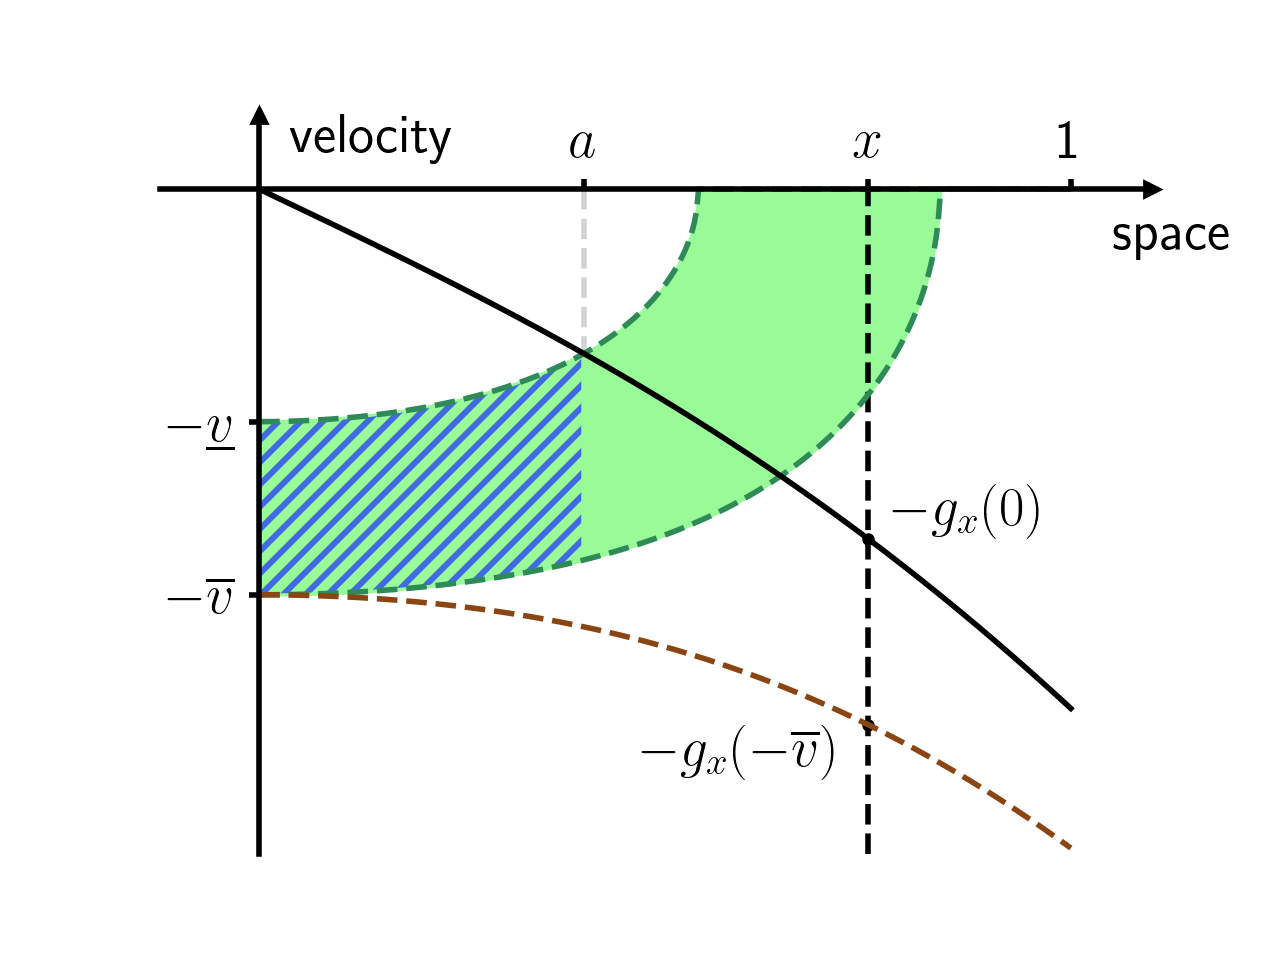
\includegraphics[width=0.5\linewidth]{images/fpcharmaps_lowerboundni}
	\caption{Notations for the lower bound on $n_i$.}
	\mysubcaption{The coloured area corresponds to the domain $\mathcal{L}_e(0,\domfel) \leqslant \mathcal{L}_e(x,v) \leqslant \mathcal{L}_e(0,\domfeu)$, on which we know that $f_e \geqslant \minfe$. The solid black line is the critical ion characteristic.}
	\label{fig:charmaps_lowerboundni}
\end{figure}

\begin{lem}
	Suppose that there exists $v_* > 0$ such that $f_{e,b}(v) = 0$ for all $|v| \leqslant v_*$. Then the density $f_i$ satisfies the uniform bound
	\begin{align*}
		f_i(x,v) \leqslant 2^{9/4} \maxfe \sqrt{\frac{\frac{\beta}{\alpha}(1+\frac{1}{\mu})+1}{v_*}} \quad \forall (x,v) \in [0,1] \times \mathbb{R}.
	\end{align*}
\end{lem}

\myproof{
	Let $(x,v) \in [0,1] \times \mathbb{R}_{-}$, and denote by $(x(t),v(t))_{t\leqslant 0}$ the ion characteristic going through $(x,v) = (x(-T),v(-T))$, with the convention $(x_b(x,v),v_b(x,v)) = (x(0),v(0))$. Owing to the positivity of $f_e$, 
	\begin{align*}
		f_i(x(0),v(0)) = \int_{t=-T}^{0} f_e(x(t),v(t)) dt + f_i(x,v) \geqslant f_i(x,v).
	\end{align*}
	On the other hand, we use $f_i(x,v) + f_i(x,-v) = 2 f_i(x(0),v(0))$ to write $f_i(x,-v) \leqslant 2 f_i(x(0),v(0))$. This shows that it is enough to bound $f_i$ on the boundary $\mathcal{B} \coloneqq \{x\geqslant0,v=0\} \cup \{x=0,v\leqslant 0\}$ to obtain an uniform bound.
	
	Let then $(x,v) \in \mathcal{B}$. By hypothesis, $f_e(x(t),v(t))$ vanishes whenever $\mathcal{L}_e(x(t),v(t)) \leqslant \mathcal{L}_e(0,v_*)$, and is bounded by $\maxfe$ otherwise. Then, we may use the reparametrization by space 
	\begin{align*}
		f_i(x,v) \leqslant \int_{z=a(x,v)}^{1} \frac{\maxfe}{\left(v^2 + 2 \varphi(x) - 2 \varphi(z)\right)^{1/2}} dz,
		\quad \text{with} \quad
		a(x,v) \coloneqq 
		\begin{cases}
			\varphi^{-1}\left(\frac{\frac{v^2}{2} + \varphi(x) - \frac{v_*^2}{2}}{1+1/\mu}\right) & \text{if } \mathcal{L}_e(x,v) \leqslant \mathcal{L}_e(0,v_*) \\
			x & \text{otherwise.}
		\end{cases}
	\end{align*}
	The function $a$ gives the smallest spatial coordinate of the characteristic $(x(t),v(t))_{t\leqslant0}$ such that $f_e > 0$. Using that $\varphi(z) \leqslant - \alpha\frac{z^2}{2}$, we have
	\begin{align*}
		f_i(x,v) \leqslant \maxfe \int_{z=a(x,v)}^{1} \frac{1}{\left(v^2 + 2 \varphi(x) - \alpha z^2\right)^{1/2}} dz \leqslant \maxfe \min\left(\frac{1}{\left|v^2 + 2 \varphi(x)\right|^{1/2}}, \frac{2}{\sqrt{\alpha a(x,v)}}\right)
	\end{align*}
	where we used \cref{lem:maj_fi} with $L\coloneqq v^2 + 2 \varphi(x)$. 
	
	We rely on the concavity estimate
	\begin{align*}
		\varphi(x) \geqslant (1 - x) \varphi(0) + x \varphi(1) + \frac{\alpha}{2} x(1-x) \geqslant - x \beta 
		\quad \implies \quad
		-\frac{y}{\beta} \leqslant \varphi^{-1}(y)
	\end{align*}
	to write that for $(x,v)$ satisfying $\mathcal{L}_e(x,v) \leqslant \mathcal{L}_e(0,v_*)$, 
	\begin{align*}
		a(x,v) = \varphi^{-1}\left(\frac{\frac{v^2}{2} + \varphi(x) - \frac{v_*^2}{2}}{1+1/\mu}\right)
		\geqslant \frac{\frac{v_*^2}{2} - (\frac{v^2}{2} + \varphi(x))}{\beta(1+1/\mu)}.
	\end{align*}
	Then 
	\begin{align*}
		f_i(x,v) \leqslant \maxfe \min \left(\frac{1}{\sqrt{|X|}}, \frac{A}{\sqrt{B - X}}\right) 
		\quad \text{with} \quad
		X \coloneqq \frac{v^2}{2} + \varphi(x), \quad A \coloneqq \frac{2}{\sqrt{\frac{\alpha}{\beta(1+1/\mu)}}}, \quad \text{and} \quad B \coloneqq \frac{v_*^2}{2}.
	\end{align*}
	 The elementary study of the function $X \to \min\left(|X|^{-1/2}, A (B-X)^{-1/2}\right)$ reveals a global maximum at $X = \frac{B}{A^2 + 1} < B$, and we conclude to the result.
	 
 	\begin{figure}
 		\centering
 		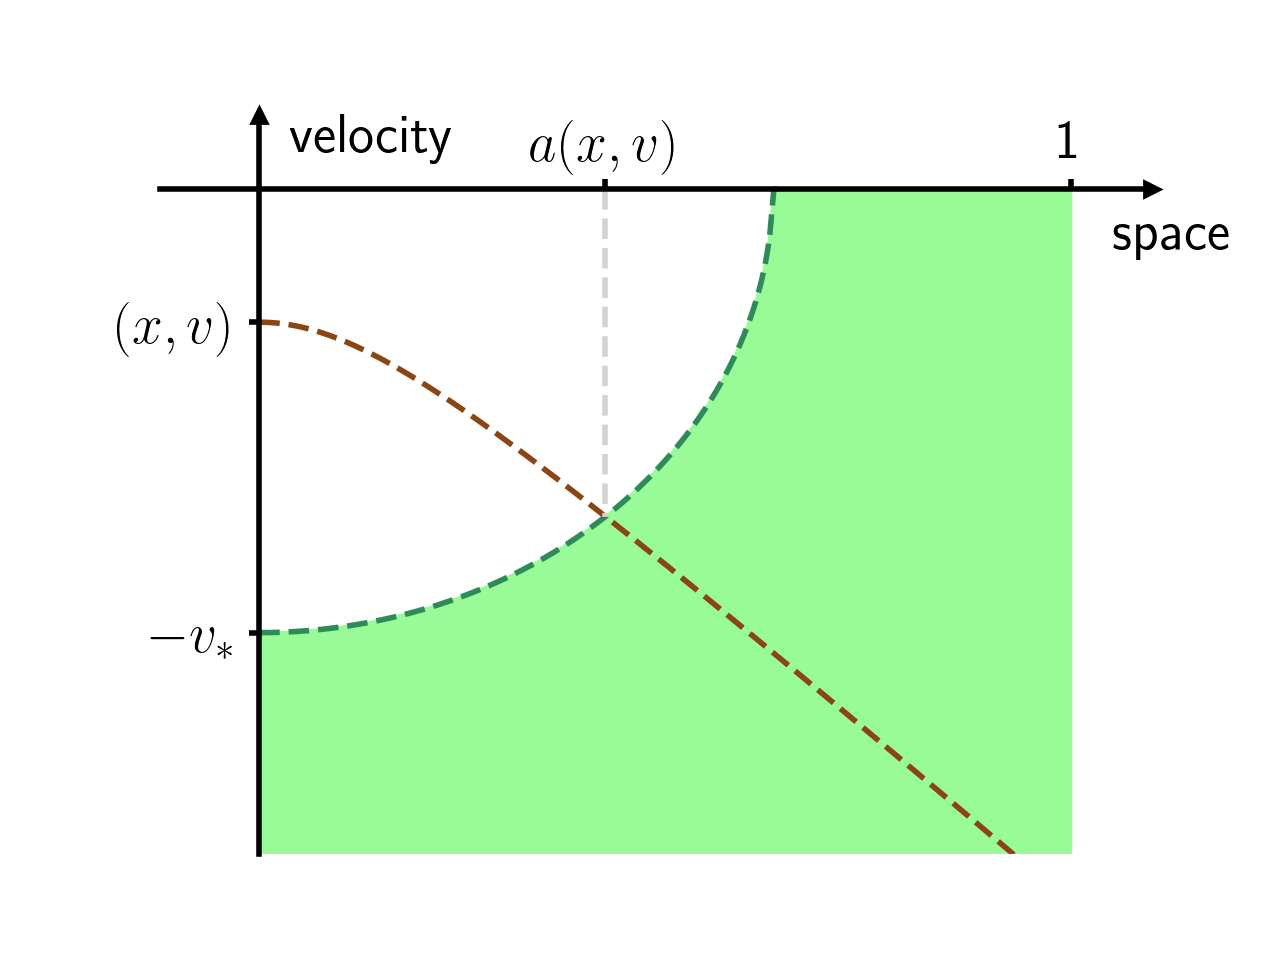
\includegraphics[width=0.5\linewidth]{images/global_bound_fi}
 		\caption{Notations for the boundedness of $f_i$.}
 		\mysubcaption{The coloured area corresponds to $\mathcal{L}_e(x,v) \geqslant \mathcal{L}_e(0,v_*)$. The function $a(x,v)$ gives the point of the ion characteristic (in brown) where $f_e$ vanishes.}
 		\label{fig:charmaps_domainmap}
 	\end{figure}
}


%%%%%%%%%%%%%%%%%%%%%%%%%%%%%%%%%%%%%%%%%%%%%%%%%%%%%%%%%%%%%%
%%%%%%%%%%%%%%%%%%%%%%%%%%%%%%%%%%%%%%%%%%%%%%%%%%%%%%%%%%%%%%
%%%% archives
%%%%%%%%%%%%%%%%%%%%%%%%%%%%%%%%%%%%%%%%%%%%%%%%%%%%%%%%%%%%%%
%%%%%%%%%%%%%%%%%%%%%%%%%%%%%%%%%%%%%%%%%%%%%%%%%%%%%%%%%%%%%%

%\subsection{Upper bounds on the densities}
%
%We want to obtain estimates on $n_i - n_e$. We make the following assumptions:
%\begin{itemize}
%\item The electron density $f_e$ satisfies the boundary condition, and is bounded by a constant $\maxfe \geqslant 0$. 
%\item The potential $\varphi$ is strongly concave, i.e. there exists $\alpha>0$ such that $\varphi''(x) \leqslant - \alpha$ uniformly over $x\in[0,1]$.
%\item We have $\varphi(0) = \varphi'(0) = 0$.
%\end{itemize}
%The assumptions on $\varphi$ yield that
%\begin{align}\label{eq:phi_concave_consequences}
%	\varphi'(x) \leqslant- \alpha x, \quad \varphi(x) \leqslant - \alpha \frac{x^2}{2}.
%\end{align}
%
%Let us first focus on $n_e(x)$. The characteristics of the electron density are the level lines of
%\begin{align}\label{eq:def_Le}
%	\mathcal{L}_e(x,v) \coloneqq \frac{v^2}{2} - \frac{1}{\mu} \varphi(x).
%\end{align}
%Since $\varphi$ is strongly concave, these curves are closed. Since $f_e$ satisfies the homogeneous boundary condition, its support is embedded in $\left\{(x,v) \ |\ \frac{v^2}{2} - \frac{1}{\mu} \varphi(x) \leqslant \frac{0^2}{2} - \frac{1}{\mu} \varphi(1)\right\}$. In particular, we denote by $\ve$ the extremal speed of the support, given by
%\begin{align}\label{eq:def_ve}
%	\ve \coloneqq \sqrt{-\frac{2}{\mu} \varphi(1)}.
%\end{align}
%We can roughly majorize
%\begin{align*}
%	n_e(x) = \int_{v\in\mathbb{R}} f_e(x,v) dv \leqslant \int_{v=-\ve}^{\ve} \maxfe dv = 2 \maxfe \ve \leqslant 2 \maxfe \sqrt{-\frac{2}{\mu} \varphi(1)}.
%\end{align*}
%
%The estimates on $n_i$ are slightly more technical. Let the ion Lyapunov function be defined as
%\begin{align}\label{eq:def_Li}
%	\mathcal{L}_i(x,v) \coloneqq \frac{v^2}{2} + \varphi(x).
%\end{align}
%In the sequel, we will heavily rely on the level lines of $\mathcal{L}_i$ to partition the space. We distinguish the \emph{critical characteristic} as the curve $\left\{\mathcal{L}_i = 0\right\}$.
%Let $x\in[0,1]$ and $v \in \mathbb{R}_{-}$. We denote by $(x_b(x,v),v_b(x,v))$ the intersection of the boundary $\left\{x=0\right\}\cap\left\{v=0\right\}$ with the characteristic issued from $(x,v)$, equal to
%\begin{align*}
%	\vv{x_b(x,v) \\ v_b(x,v)} \coloneqq 
%	\begin{cases}
%		\vv{\varphi^{-1}\left(\frac{v^2}{2} + \varphi(x)\right) \\ 0} & \text{if } \mathcal{L}_i(x,v) \leqslant 0, \\
%		\vv{0 \\ - \sqrt{\frac{v^2}{2} + \varphi(x)}} & \text{if } \mathcal{L}_i(x,v) > 0.
%	\end{cases}
%\end{align*}
%In the following paragraph, we use $(x(t),v(t))_{t\leqslant0}$ to denote the characteristic reaching $(x_b(x,v),v_b(x,v))$ at $t=0$. 
%We use the symmetry of $f_i$ to write 
%\begin{align*}
%	n_i(x) = 2 \int_{v\in\mathbb{R}^{-}} f_i(x_b(x,v), v_b(x,v)) dv = 2 \int_{v\in\mathbb{R}^{-}}\int_{t=-\infty}^{0} f_e(x(t),v(t)) dt dv.
%\end{align*}
%The lower bound $t \to -\infty$ is artificial, since the characteristic exits the support of $f_e$ in finite time. We will split the double integral in three domains:
%\begin{enumerate}
%\item $\DomUpL$ will be $\left\{(v,t) \in \mathbb{R}_{-}^2 \ |\ \mathcal{L}_i(x,v) \leqslant 0 \text{ and } x(t) \leqslant x \right\}$. This is the region contained between the $x-$axis, the critical characteristic and the vertical line going through $x$.
%\item $\DomUpR$ is $\left\{(v,t) \in \mathbb{R}_{-}^2 \ |\ \mathcal{L}_i(x,v) \leqslant 0 \text{ and } x < x(t) \leqslant 1 \right\}$. It cover the part of the domain intersecting $\left\{\mathcal{L}_i \leqslant 0\right\} \setminus \DomUpL$.
%\item $\DomLow$ is defined by $\left\{(v,t) \in \mathbb{R}_{-}^2 \ |\ \mathcal{L}_i(x,v) > 0 \text{ and } -\ve \leqslant v(t) \right\}$. 
%\end{enumerate}
%The corresponding phase space decomposition is represented in \cref{fig:charmaps_domainmap}.
%
%\begin{figure}
%	\centering
%	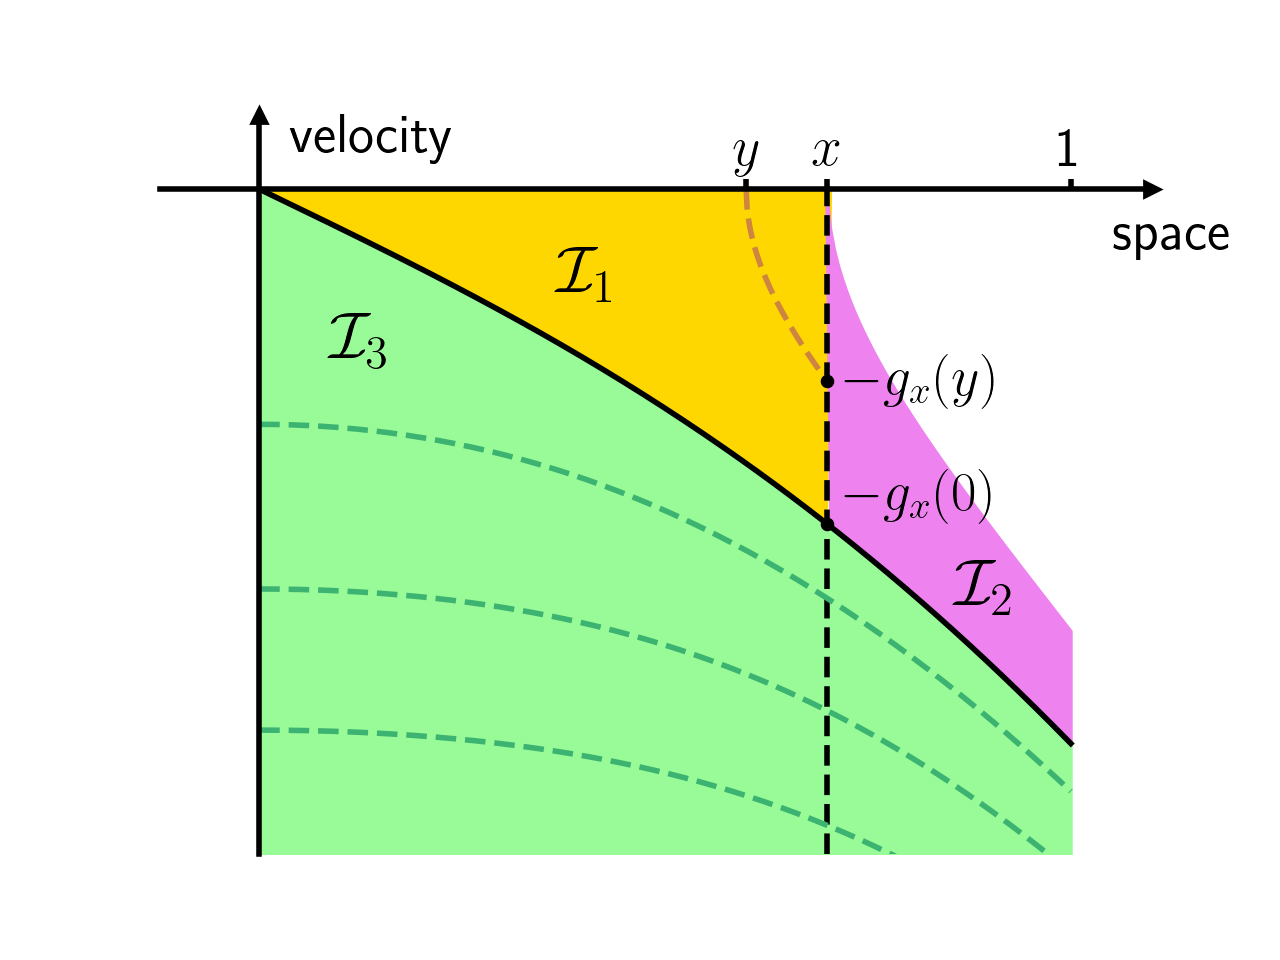
\includegraphics[width=0.5\linewidth]{images/fpcharmaps_domainmap}
%	\caption{Representation in the phase space $(x,v)$ of the decomposition of $(x,t)\in\mathbb{R}_-^2$ in $\DomUpL\cup\DomUpR \cup \DomLow$.}
%	\label{fig:charmaps_domainmap}
%\end{figure}
%
%Since $f_e(x(t),v(t))$ vanishes outside $\DomUpL \cup \DomUpR \cup \DomLow$, we may exactly decompose $n_i$ in 
%\begin{align*}
%	\frac{n_i(x)}{2} = \underbrace{\iint_{(v,t) \in \DomUpL} f_e(x(t),v(t)) dt dv}_{\IntUpL} + \underbrace{\iint_{(v,t) \in \DomUpR} f_e(x(t),v(t)) dt dv}_{\IntUpR} + \underbrace{\iint_{(v,t) \in \DomLow} f_e(x(t),v(t)) dt dv}_{\IntLow} 
%\end{align*}
%
%Each term will be bound separately. 
%
%\paragraph{Bound on $\IntUpL$}
%
%Let $v_0(x) \coloneqq \sqrt{-2\varphi(x)}$ be the velocity such that $(x, -v_0(x))$ belongs to the critical characteristic. 
%The characteristics in the domain $\DomUpL$ are joining points $(x,v)$, with $v \in [-v_0(x),0]$, with points $(x_b(x,v), 0)$. Therefore, we may use the reparametrization 
%\begin{align*}
%	y = x(t), \quad dy = \dot{x}(t) dt = v(t) dt = - \left(v^2 + 2 \left(\varphi(x) - \varphi(x(t))\right)\right)^{1/2} dt = - \left(v^2 + 2 \left(\varphi(x) - \varphi(y)\right)\right)^{1/2} dt	
%\end{align*}
%The integral $\IntUpL$ becomes
%\begin{align*}
%	\IntUpL = \int_{v=-v_0(x)}^0 \int_{y=x}^{x_b(x,v)} f_e(y,- \left(v^2 + 2 \left(\varphi(x) - \varphi(y)\right)\right)^{1/2}) \frac{-1}{\left(v^2 + 2 \left(\varphi(x) - \varphi(y)\right)\right)^{1/2}} dy dv.
%\end{align*}
%By exchanging the bounds of the integrals along $y$, and using $f_e \leqslant \maxfe$, we get
%\begin{align*}
%	\IntUpL \leqslant \maxfe \int_{v=-v_0(x)}^0 \int_{y=x_b(x,v)}^{x} \frac{1}{\left(v^2 + 2 \left(\varphi(x) - \varphi(y)\right)\right)^{1/2}} dy dv.
%\end{align*}
%In order to use the explicit $v^2$, we use Fubini theorem to switch the order of integration (since everything is positive). To do this, we write
%\begin{align*}
%	\begin{cases}
%		- v_0(x) \leqslant v \leqslant 0 \\
%		x_b(x,v) \leqslant y \leqslant x 
%	\end{cases}
%	\quad \iff \quad 
%	\begin{cases}
%		0 \leqslant y \leqslant x \\
%		- v_0(x) \leqslant v \leqslant - g_x(y)
%	\end{cases}
%\end{align*}
%where $y = x_b(x,v) = \varphi^{-1}\left(\frac{v^2}{2} + \varphi(x)\right)$ is equivalent to $v = - g_x(y) \coloneqq - \left(2\left(\varphi(y) - \varphi(x)\right)\right)^{1/2}$. In the sequel, we drop the $x$ and simply write $g(y)$. The function $g : [0,x] \mapsto \mathbb{R}^{+}$ is well-defined, since $y \leqslant x \implies \varphi(y) \geqslant \varphi(x)$. By the assumption of strong concavity of $\varphi$, $g$ is positive whenever $y < x$. Finally, using that $v_0(x) = g(0)$, may now write 
%\begin{align*}
%	\IntUpL \leqslant \maxfe \int_{y=0}^{x} \int_{v=-v_0(x)}^{-g(y)}  \frac{1}{\left(v^2 - g^2(y)\right)^{1/2}} dv dy \underset{\text{with }w\coloneqq g(y)-v}{=} \maxfe \int_{y=0}^{x} \int_{w=0}^{g(0)-g(y)}  \frac{1}{\left(w^2 + 2 w g(y)\right)^{1/2}} dv dy.
%\end{align*}
%By integration with $\frac{d}{dy} [\sinh^{-1}\left(\sqrt{\frac{y}{a}}\right)] = \frac{1}{(y^2 + 2 a y)^{1/2}}$, we obtain
%\begin{align*}
%	\IntUpL \leqslant \maxfe \int_{y=0}^{x} \left[\sinh^{-1}\left(\sqrt{\frac{v}{g(y)}}\right)\right]^{g(0)-g(y)}_{0} dv = \maxfe \int_{y=0}^{x} \sinh^{-1}\left(\sqrt{\frac{g(0)-g(y)}{g(y)}}\right) dv.
%\end{align*}
%We use the coarse estimates $\sinh^{-1}(z) \leqslant z$ and $\sqrt{\frac{a-b}{b}} \leqslant \sqrt{\frac{a}{b}}$ to reduce the expression to
%\begin{align*}
%	\IntUpL \leqslant \maxfe \sqrt{g(0)} \int_{y=0}^{x} \frac{1}{\sqrt{g(y)}} dv = \maxfe \sqrt{g(0)} \int_{y=0}^{x} \frac{1}{\left(2\left(\varphi(y) - \varphi(x)\right)\right)^{1/4}} dv.
%\end{align*}
%Using the strong concavity of $\varphi$, and the sign $-\varphi'(y) \geqslant 0$, we get
%\begin{align*}
%	\varphi(y) - \varphi(x) \geqslant \frac{\alpha}{2} |x - y|^2 - \varphi'(y)(x-y) \geqslant \frac{\alpha}{2} (x - y)^2.
%\end{align*}
%With this, we may finally write
%\begin{align*}
%	\IntUpL \leqslant \maxfe \sqrt{g(0)} \int_{y=0}^{x} \frac{1}{\alpha^{1/4}\left(x-y\right)^{1/2}} dv = \frac{2 \maxfe}{\alpha^{1/4}} \sqrt{g(0) x} = \frac{2 \maxfe}{\alpha^{1/4}} \sqrt{\sqrt{-2\varphi(x)} x} \leqslant \frac{2 \maxfe}{\alpha^{1/4}} \left(-2\varphi(1)\right)^{1/4}.
%\end{align*}
%
%\paragraph{Bound on $\IntUpR$}
%
%We use the same reparametrization as for $\IntUpR$, but with $y \in [x,1]$, to obtain
%\begin{align*}
%	\IntUpR \leqslant \maxfe \int_{v=-v_0(x)}^{0} \int_{y=x}^{1} \frac{1}{\left(v^2 + 2(\varphi(x) - \varphi(y))\right)^{1/2}} dy dv.
%\end{align*}
%On $y \geqslant x$, we may directly use
%\begin{align*}
%	\varphi(x) - \varphi(y) \geqslant \frac{\alpha}{2} |y - x|^2 - \varphi'(x) (y-x) \geqslant \frac{\alpha}{2} (y - x)^2
%\end{align*}
%to get
%\begin{align*}
%	\IntUpR \leqslant \maxfe \int_{v=-v_0(x)}^{0} \int_{y=x}^{1} \frac{1}{\left(v^2 + \alpha(y-x)^2\right)^{1/2}} dy dv \leqslant \maxfe \max\left(1,\frac{1}{\sqrt{\alpha}}\right) \int_{v=0}^{v_0(x)} \int_{z=0}^{1-x} \frac{1}{\left(v^2 + z^2\right)^{1/2}} dy dv.
%\end{align*}
%By switching to polar coordinates over the (larger) domain $(\theta,r) \in [0,\frac{\pi}{2}] \times [0,\sqrt{v_0(x)^2 + (1-x)^2}]$, we conclude to 
%\begin{align*}
%	\IntUpR \leqslant \maxfe \max\left(1,\frac{1}{\sqrt{\alpha}}\right) \frac{\pi}{2} \sqrt{v_0(x)^2 + (1-x)^2} \leqslant \maxfe \max\left(1,\frac{1}{\sqrt{\alpha}}\right) \frac{\pi}{2} \sqrt{1 - 2\varphi(1)}.
%\end{align*} 
%
%\paragraph{Bound on $\IntLow$}
%
%The domain $\DomLow$ is covered by characteristics linking $x=1$ to $x=0$. We may use the same reparametrization within fixed bounds over $y$:
%\begin{align*}
%	\IntLow \leqslant \maxfe \int_{v=-\ve}^{-v_0(x)} \int_{y=0}^{1} \frac{1}{\left(v^2 + 2 \left(\varphi(x) - \varphi(y)\right)\right)^{1/2}} dy dv = \maxfe \int_{y=0}^{1} \int_{v=-\ve}^{-v_0(x)} \frac{1}{\left(v^2 + 2 \left(\varphi(x) - \varphi(y)\right)\right)^{1/2}} dy dv.
%\end{align*}
%We will use the same argument as for $\IntUpR$, but with characteristics ending on $x=0$ instead of $x=x$. Our first step is then to replace $v$ by $w$ the velocity at $x=0$, defined by $\frac{v^2}{2} + \varphi(x) = \frac{w^2}{2} + 0$. We have
%\begin{align*}
%	 w = - \left(v^2 + 2 \varphi(x)\right)^{1/2} \in [-\we, 0], \quad v = - \left(v^2 - 2 \varphi(x)\right)^{1/2}, \quad dv = \frac{-w}{\left(w^2-2\varphi(x)\right)^{1/2}} dw,
%\end{align*}
%where $\we \coloneqq \left(\ve^2 + 2 \varphi(x)\right)^{1/2} \leqslant \ve \leqslant \sqrt{-2\varphi(1)}$. Using the estimate $-\varphi(y) \geqslant \alpha \frac{y^2}{2}$, we conclude similarly that
%\begin{align*}
%	\IntLow 
%	\leqslant \maxfe \int_{y=0}^{1} \int_{w=-\we}^{0} \frac{1}{\left(w^2 - 2\varphi(y)\right)^{1/2}} dy dv 
%	= \maxfe \int_{y=0}^{1} \int_{w=0}^{\we} \frac{1}{\left(w^2 + \alpha y^2\right)^{1/2}} dy dv
%	\leqslant \maxfe \max\left(1,\frac{1}{\sqrt{\alpha}}\right) \frac{\pi}{2} \sqrt{1 - 2 \varphi(1)}.
%\end{align*}
%
%In conclusion, we obtained the uniform bound
%\begin{align*}
%	n_i(x) \leqslant \frac{4}{\alpha^{1/4}} \left(-2\varphi(1)\right)^{1/4} + 4 \maxfe \max\left(1,\frac{1}{\sqrt{\alpha}}\right) \frac{\pi}{2} \sqrt{1 - 2 \varphi(1)}.
%\end{align*}
%
%\subsection{Lower bound on $n_i$}
%
%Let us consider that $f_{e,b}$ is positive on a segment. More precisely, we assume that there exists $0 \leqslant \domfel < \domfeu \leqslant \ve$ and $\minfe > 0$ such that $f_e([-\domfeu,-\domfel]) \geqslant \minfe$.
%The value $\minfe$ is propagated along every electron characteristic crossing $(x=0,v\in[-\domfeu,-\domfel])$, so that we may use the lower estimate
%\begin{align*}
%	f_e(x,v) \geqslant \minfe \,\textbf{1}_{\left\{\mathcal{L}_e(0,\domfel) \leqslant \mathcal{L}_e(x,v) \leqslant \mathcal{L}_e(0,\domfeu)\right\}}.
%\end{align*}
%Let us parametrize the electron characteristic issued from $(0,-\domfeu)$ by $(\overline{y}(v), v)$, with $v\in[-\domfeu,0]$. Let $x\in[0,1]$, and define $\underline{w}$ and $\overline{w}$ by
%\begin{align*}
%	\begin{cases}
%		\mathcal{L}_i(0,-\domfeu) = \mathcal{L}_i(x,-\underline{w}), \\
%		\mathcal{L}_i(0,-\domfel) = \mathcal{L}_i(x,-\overline{w})
%	\end{cases}
%	\quad \text{that is} \quad
%	\begin{cases}
%		\underline{w} \coloneqq \left(\frac{\domfeu^2}{2} - 2 \varphi(x)\right)^{1/2} \\
%		\overline{w} \coloneqq \left(\frac{\domfel^2}{2} - 2 \varphi(x)\right)^{1/2}
%	\end{cases}
%\end{align*}
%
%\begin{figure}
%	\centering
%	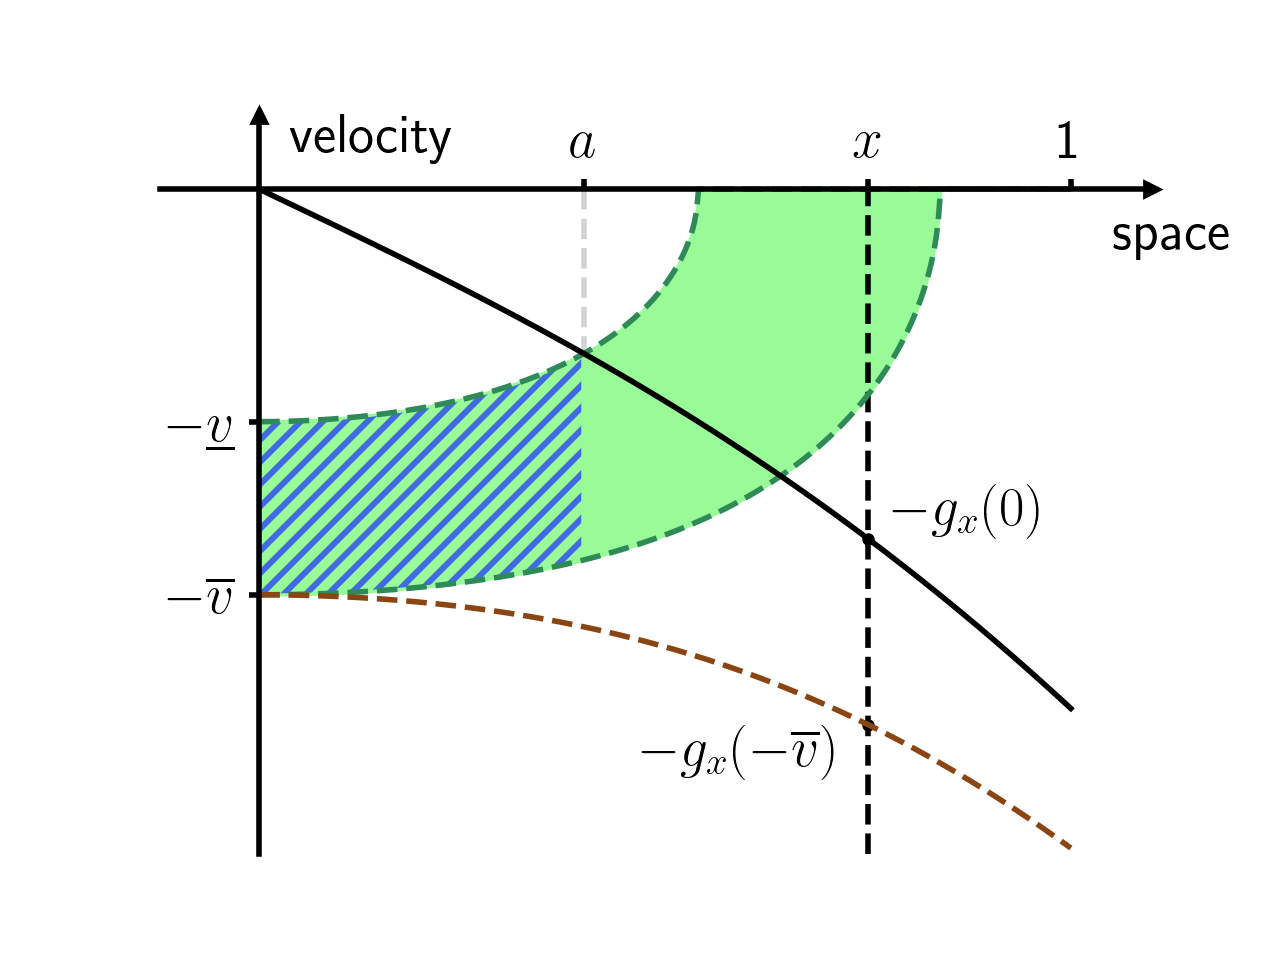
\includegraphics[width=0.5\linewidth]{images/fpcharmaps_lowerboundni}
%	\caption{Notations for the lower bound on $n_i$.}
%	\mysubcaption{The coloured area corresponds to the domain $\mathcal{L}_e(0,\domfel) \leqslant \mathcal{L}_e(x,v) \leqslant \mathcal{L}_e(0,\domfeu)$, on which we know that $f_e \geqslant \minfe$. The parametrization $(\overline{y}(w),w)$ of the electron characteristic crossing $(0,-\domfeu)$ is equivalent to $(y,-h(y))$.}
%	\label{fig:charmaps_lowerboundni}
%\end{figure}
%
%Then, using the (now classical) reparametrization, the ion density satisfies
%\begin{align*}
%	n_i(x) \geqslant \minfe \int_{w=-\overline{w}}^{-\underline{w}} \int_{y=0}^{\overline{y}(w)} \frac{1}{\left(w^2 + 2\left(\varphi(x) - \varphi(y)\right)\right)^{1/2}} dy dw.
%\end{align*}
%As for the integral $\IntLow$, we wish to use the velocity at $x=0$ instead of $x=x$. We define $v\in[-\domfeu,-\domfel]$ by
%\begin{align*}
%	\mathcal{L}_i(0,v) = \mathcal{L}_i(x,w), \quad w = - \left(v^2 - 2 \varphi(x)\right)^{1/2}, \quad dw = \frac{- v}{\left(v^2 - 2 \varphi(x)\right)^{1/2}}.
%\end{align*}
%This yields
%\begin{align*}
%	n_i(x) \geqslant \minfe \int_{v=-\domfeu}^{-\domfel} \int_{y=0}^{\overline{y}(w(v))} \frac{1}{\left(v^2 - 2\varphi(y)\right)^{1/2}} dy  \frac{-v}{\left(v^2 - 2 \varphi(x)\right)^{1/2}} dv.
%\end{align*}
%The upper bound $\overline{y}(w(v))$ is equal to $\varphi^{-1}\left(\frac{\mu}{2}\left(v^2 - \domfeu^2\right)\right)$.
%Since $-\varphi(z) \leqslant -\varphi(1)$ for all $z$, this gives
%\begin{align*}
%	n_i(x) \geqslant \minfe \int_{v=-\domfeu}^{-\domfel} \overline{y}(w(v)) \frac{-v}{v^2 - 2\varphi(1)} dv = \minfe \int_{v=-\domfeu}^{-\domfel} \varphi^{-1}\left(\frac{\mu}{2}\left(v^2 - \domfeu^2\right)\right) \frac{-v}{v^2 - 2\varphi(1)} dv.
%\end{align*}
%
%Let $v_* \in ]\domfel,\domfeu[$ be the velocity such that $v_*^2 - \domfel^2 = \frac{\domfeu^2 - \domfel^2}{2}$. We split the integral on $[-\domfeu,-v_*[ \cup [-v_*,\domfel]$ and use the decreasing monotonicity of $\varphi^{-1}$ to write
%\begin{align*}
%	n_i(x) 
%	&\geqslant 0 + \varphi^{-1}\left(\frac{\mu}{2}\left(v_*^2 - \domfeu^2\right)\right) \minfe \int_{v=-v_*}^{-\domfel} \frac{-v}{v^2 - 2\varphi(1)} dv \\
%	&= \frac{\minfe}{2} \varphi^{-1}\left(\frac{\mu}{4}\left(\domfel^2 - \domfeu^2\right)\right) \log\left(\frac{v_*^2 - 2 \varphi(1)}{\domfel^2 - 2 \varphi(1)}\right) \\
%	&\geqslant \frac{\minfe}{2} \varphi^{-1}\left(\frac{\mu}{4}\left(\domfel^2 - \domfeu^2\right)\right) \log\left(1 + \frac{\domfeu^2 - \domfel^2}{\domfel^2 - 2 \varphi(1)}\right).
%\end{align*}

%\bibliographystyle{alpha}
%\bibliography{CEMRACS.bib}

\end{document}